\documentclass{ExcelAtFIT}
%\documentclass[czech]{ExcelAtFIT} % when writing in CZECH
%\documentclass[slovak]{ExcelAtFIT} % when writing in SLOVAK


%--------------------------------------------------------
%--------------------------------------------------------
%	REVIEW vs. FINAL VERSION
%--------------------------------------------------------

%   LEAVE this line commented out for the REVIEW VERSIONS
%   UNCOMMENT this line to get the FINAL VERSION
%\ExcelFinalCopy


%--------------------------------------------------------
%--------------------------------------------------------
%	PDF CUSTOMIZATION
%--------------------------------------------------------

\hypersetup{
	pdftitle={ENOSS},
	pdfauthor={Nemanja Vasiljević},
	pdfkeywords={Event, Notifications, OpenStack Swift}
}

\lstset{
	backgroundcolor=\color{white},   % choose the background color; you must add \usepackage{color} or \usepackage{xcolor}; should come as last argument
	basicstyle=\footnotesize\tt,        % the size of the fonts that are used for the code
}

\definecolor{darkpastelred}{rgb}{0.76, 0.23, 0.13}
\definecolor{codegray}{rgb}{0.5,0.5,0.5}
\definecolor{codepurple}{rgb}{0.58,0,0.82}
\definecolor{backcolour}{rgb}{0.95,0.95,0.92}
\lstdefinestyle{pythonStyle}{
    backgroundcolor=\color{backcolour},
    commentstyle=\color{codegreen},
    keywordstyle=\color{blue},
    numberstyle=\tiny\color{codegray},
    stringstyle=\color{codepurple},
    basicstyle=\ttfamily\footnotesize,
    breakatwhitespace=false,
    breaklines=true,
    captionpos=b,
    keepspaces=true,
    numbers=right,
    showspaces=false,
    showstringspaces=false,
    showtabs=false,
    tabsize=2
}
\lstdefinestyle{jsonStyle}{
    string=[s]{"}{"},
    stringstyle=\color{darkpastelred},
    comment=[l]{:},
    breaklines=true,
    commentstyle=\color{black},
    captionpos=b
}

%--------------------------------------------------------
%--------------------------------------------------------
%	ARTICLE INFORMATION
%--------------------------------------------------------

\ExcelYear{2022}

\PaperTitle{ENOSS - Event Notifications in OpenStack Swift}

\Authors{Nemanja Vasiljević*}
\affiliation{*%
  \href{mailto:xvasil03@stud.fit.vutbr.cz}{xvasil03@stud.fit.vutbr.cz},
  \textit{Faculty of Information Technology, Brno University of Technology}}
%%%%--------------------------------------------------------
%%%% in case there are multiple authors, use the following fragment instead
%%%%--------------------------------------------------------
%\Authors{Jindřich Novák*, Janča Dvořáková**}
%\affiliation{*%
%  \href{mailto:xnovak00@stud.fit.vutbr.cz}{xnovak00@stud.fit.vutbr.cz},
%  \textit{Faculty of Information Technology, Brno University of Technology}}
%\affiliation{**%
%  \href{mailto:xdvora00@stud.fit.vutbr.cz}{xdvora00@stud.fit.vutbr.cz},
%  \textit{Faculty of Information Technology, Brno University of Technology}}

\Keywords{Event --- Notifications --- OpenStack Swift}

\Supplementary{\href{https://github.com/xvasil03/master-thesis/tree/main/src}{Github repository}}


%--------------------------------------------------------
%--------------------------------------------------------
%	ABSTRACT and TEASER
%--------------------------------------------------------

\Abstract{

%What is the problem? What is the topic?, the aim of this paper?
Currently, object storage OpenStack Swift does not provide any pieces of information to users about events that occurred in storage they own/have access to. For example, users do not have information when the content of their object storage is accessed, changed, created, or deleted.
This paper aims to create a solution that will send notifications about events that occurred in OpenStack Swift to user-specified destinations.
%How is the problem solved, the aim achieved (methodology)?
The proposed solution, using metadata, allows users to specify where and which event should be published based on even types (read, create, modify, delete) and other properties such as object prefix, suffix, size. It also offers multiple destinations(Beanstalkd queue, Kafka, etc.) to which notifications can be published.
%What are the specific results? How well is the problem solved?
The solution is fully compatible with AWS S3 Event Notifications and, compared to AWS, supports more destinations, event types, filters and allows unsuccessful events to be published.
%So what? How useful is this to Science and to the reader?
Event notification can be used for monitoring, automatization, and serverless computing (similar to AWS Lambda).
}


\Teaser{
	\TeaserImage{swift-logo.png}
	\TeaserImage{automation.png}
	\TeaserImage{lambda.pdf}
	\TeaserImage{monitoring.pdf}
}



%--------------------------------------------------------
%--------------------------------------------------------
%--------------------------------------------------------
%--------------------------------------------------------
\begin{document}

\startdocument


%--------------------------------------------------------
%--------------------------------------------------------
%	ARTICLE CONTENTS
%--------------------------------------------------------

%--------------------------------------------------------
%--------------------------------------------------------
%--------------------------------------------------------
%--------------------------------------------------------
\section{Introduction} \label{sec:introduction}

% Questions to answer:
% - why now? skip?
% - why this? skip??
% - why this way?
% - why should reader care?
% Important: Story telling!


%\textbf{[Motivation]} What is the raison d'\^{e}tre of your project? Why should anyone care? No general meaningless claims. Make bulletproof arguments for the importance of your work.

Object storage is a data storage architecture that manages data as objects, and each object typically includes data itself and some additional information stored in objects metadata. Since object storage is often used in cloud computing, data are stored in remote locations where users do not have direct and complete access. Some users or external services might want to receive information about specific events in storage where their data are located. For example, there is no easy way to detect changes in a specific container except to list its content and compare timestamps, which can be complex, slow, and inefficient if there are many objects in storage.

The importance of this work is to provide event information to users in OpenStack Swift, which will allow users to react to those events, create more sophisticated backend operations, postprocessing and automatization, or possibly prevent/detect unwanted actions. In addition, providing event notifications will allow users to have a better picture of what is going on in their storage and improve monitoring in object storage.

%\textbf{[Problem definition]} What exactly are you solving? What is the core and what is a bonus? What parameters should a proper solution of the problem have? Define the problem precisely and state how its solution should be evaluated.

Users can be interested in only specific events, for example, creating new objects in the container. Therefore, the proposed solution must allow event filtering based on event type and other properties (e.g., object name prefix/suffix/size). Furthermore, since object storage has multiple users, each user can have different requirements for event notification, and the proposed solution must be prepared for it.

Application of event notifications varies from simple monitoring or webhook to more sophisticated applications such as serverless computing like AWS Lambda. Therefore the structure of event notification may differ based on the application and destination to which it is published. Therefore, the proposed solution must be ready to publish event notifications to different destinations and event notification structures.

AWS S3 object storage is one of the most popular storage with their API, supported by many other object storages, including OpenStack Swift. Since AWS S3 supports event notifications, it would be ideal if the proposed solution in OpenStack is compatible with the S3 event notification protocol. As a result, not only that OpenStack Swift would offer the same functionality as AWS S3 (that currently lacks), but the protocol would be compatible with AWS S3, which would allow more accessible transfer users from AWS S3 to OpenStack Swift. Therefore, users would not have to learn additional protocols, instead can follow the existing AWS S3, which is most popular and well documented.

This work consists of six chapters. Chapter \ref{sec:introduction} introduces the motivation, defines problems and desired objectives. Chapter \ref{sec:swift} describes object storage OpenStack Swift, its data model, main processes, and describes middlewares and metadata within OpenStack Swift. Chapter \ref{sec:existingSolutions} analyzes and compares existing solution for given problem. Chapter \ref{sec:ENOSS} describes proposed solution - ENOSS, its key features, configuration and interfaces. Chapter \ref{sec:conclusions} summarize proposed solution, highlights results of this work and its contributions. Chapter \ref{sec:ackn} contains acknowledgments to people that helped me to create this paper.

\section{OpenStack Swift}\label{sec:swift}

OpenStack Swift is open-source object storage developed by Rackspace, a company that, together with NASA, created the OpenStack project. After becoming an open-source project, Swift became the leading open-source object storage supported and developed by many famous IT companies, such as Red Hat, HP, Intel, IBM, and others.

OpenStack Swift is a multi-tenant, scalable, and durable object storage capable of storing large amounts of unstructured data at low cost\cite{swiftOpenStackSwift}.

\subsection{Data model}

OpenStack Swift allows users to store unstructured data objects with a canonical name containing \textit{account}, \textit{container} and \textit{object} in given order\cite{swiftOpenStackSwift}. The account names must be unique in the cluster, the container name must be unique in the account space, and the object names must be unique in the container. Other than that, if containers have the same name but belong to a different account, they represent different storage locations. The same principle applies to objects. If objects have the same name but not the same container and account name, then these objects are different.

\textbf{Accounts} are root storage locations for data. Each account contains a list of containers within the account and metadata stored as key-value pairs. Accounts are stored in the account database. In OpenStack Swift, account is \textbf{storage account} (more like storage location) and \textbf{do not represent a user identity}\cite{swiftOpenStackSwift}.

\textbf{Containers} are user-defined storage locations in the account namespace where objects are stored. Containers are one level below accounts; therefore, they are not unique in the cluster. Each container has a list of objects within the container and metadata stored as key-value pairs. Containers are stored in container database\cite{swiftOpenStackSwift}.

\textbf{Objects} represent data stored in OpenStack Swift. Each object belongs to one (and only one) container. An object can have metadata stored as key-value pairs. Swift stores multiple copies of an object across the cluster to ensure durability and availability. Swift does this by assigning an object to \textit{partition}, which is mapped to multiple drives, and each driver will contain object copy\cite{swiftOpenStackSwift}.


\subsection{Main processes}
The path towards data in OpenStack Swift consists of four main software services: \textbf{Proxy server}, \textbf{Account server}, \textbf{Continaer server} and \textbf{Object server}. Typically Account, Container and Object server are located on same machine creating \textbf{Storage node}.

\textbf{Proxy server} is the service responsible for communication with external clients. For each request, it will look up storage location(node) for an account, container, or object and route the request accordingly\cite{SwiftArchitecturalOverview}. The proxy server is responsible for handling many failures. For example, when a client sends a \texttt{PUT} request to OpenStack Swift, the proxy server will determine which nodes store the object. If some node fails, a proxy server will choose a hand-off node to write data. When a majority of nodes respond successfully, then the server proxy will return a success response code\cite{swiftOpenStackSwift}.

\textbf{Account server} stores information about containers in a particular account to SQL database. It is responsible for listing containers. It does not know where specific containers are, just what containers are in an account\cite{SwiftArchitecturalOverview}.

\textbf{Container server} is similar to the account server, except it is responsible for listing objects and also does not know where specific objects are\cite{SwiftArchitecturalOverview}.

\textbf{Object Server} is blob storage capable of storing, retrieving, and deleting objects. Objects are stored as binary files to a filesystem, where metadata are stored in the \textit{file's extended attributes (xattrs)}. This requires a filesystem with support of such attributes. Each object is stored using a hash value of object path (account/container/object) and timestamp. This allows storing multiple versions of an object. Since last write wins (due to timestamp), it is ensured that the correct object version is served\cite{SwiftArchitecturalOverview}.

\begin{figure}[t]
		\centering
		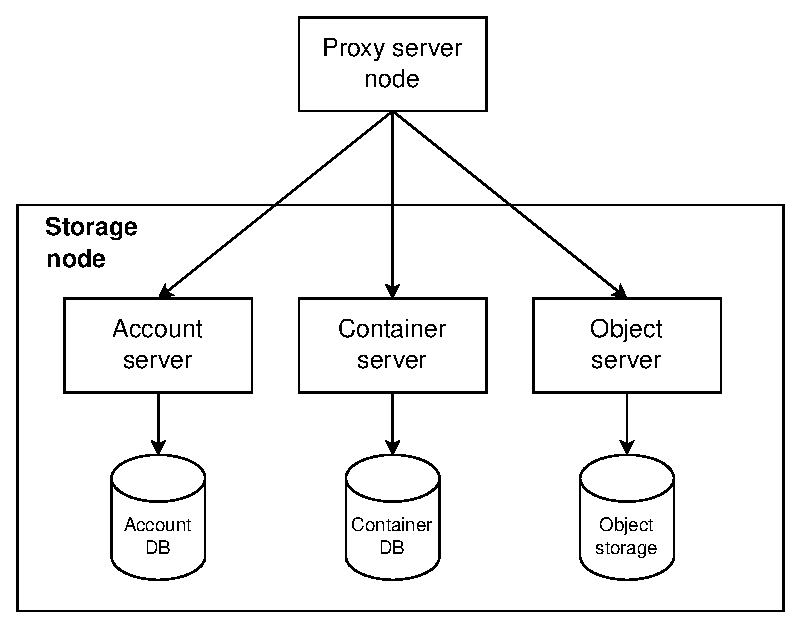
\includegraphics[width=0.90\linewidth]{images/swift-servers.eps}
		\caption{OpenStack Swift servers architecture.}
		\label{fig:swiftServers}
\end{figure}


\subsection{Middleware}\label{sbs:swiftMiddleware}
Using Python WSGI middleware, users can add functionalities and behaviors to OpenStack Swift. Most middlewares are added to the Proxy server but can also be part of other servers (account server, container server, or object server).

Middlewares are added by changing the configuration of servers. Listing \ref{lst:swiftMiddleware} is shows how to add \textit{webhook middleware} to proxy server by changing its pipeline (\textit{pipeline:main}). Middlewares are executed in the given order (first will be called webhook middleware, then proxy-server middleware).

Some of the middlewares are required and will be automatically inserted by swift code\cite{swiftMiddleware}.

\lstset{
		caption=Example of proxy server configuration (proxy-server.conf).,
		label=lst:swiftMiddleware
}
\begin{lstlisting}
[DEFAULT]
log_level = DEBUG
user = <your-user-name>

[pipeline:main]
pipeline = webhook proxy-server

[filter:webhook]
use = egg:swift#webhook

[app:proxy-server]
use = egg:swift#proxy
\end{lstlisting}

\textbf{Interface} - OpenStack Swift servers are implemented using Python WSGI applications. Therefore only Python WSGI middlewares are accepted in OpenStack Swift.

Listing \ref{lst:swift-healthcheck} provides example of simplified \textit{healthcheck middleware}. The constructor takes two arguments, the first is a WSGI application, and the second is a configuration of middleware defined using Python Paste framework in \textit{proxy-server.conf}. Middleware must have a call method containing the request environment information and response from previously called middleware. Middleware can perform some operations and call the next middleware in the pipeline or intercept a request. In the healthcheck example, if the path directs to \texttt{/healthcheck} , the middleware will return \texttt{HTTP Response}, and other middlewares in the pipeline will not be called.

Method \texttt{filter\_factory} is used by the Python Paste framework to instantiate middleware.

\begin{lstlisting}[language=Python, style=pythonStyle, caption=Example of healthcheck middleware in OpenStack Swift, label=lst:swift-healthcheck]
import os
from swift.common.swob import Request, Response

class HealthCheckMiddleware(object):
  def __init__(self, app, conf):
    self.app = app

  def __call__(self, env, start_response):
    req = Request(env)
    if req.path == '/healthcheck':
      return Response(request=req, body=b"OK", content_type="text/plain")(env, start_response)
    return self.app(env, start_response)

def filter_factory(global_conf, **local_conf):
  conf = global_conf.copy()
  conf.update(local_conf)

  def healthcheck_filter(app):
    return HealthCheckMiddleware(app, conf)
  return healthcheck_filter
\end{lstlisting}

\subsection{Metadata}
OpenStack Swift separates metadata into 3 categories based on their use:

\textbf{\texttt{User Metadata}} - User metadata takes form \\
\centerline{\texttt{X-<type>-Meta-<key>:<value>}}\\ where \texttt{<type>} represent resource type(i.e. account, container, object), and \texttt{<key>} and \texttt{<value>} are set by user. User metadata remain persistent until are updated using new value or removed using header \texttt{X-<type>-Meta-<key>} with no value or a header \texttt{X-Remove-<type>-Meta-<key>:<ignored-\\-value>}.

\textbf{\texttt{System Metadata}} - System metadata takes form \texttt{X-<type>-Sysmeta-<key>:<value>}\\ where \texttt{<type>} represent resource type(i.e. account, container, object) and \texttt{<key>} and \texttt{<value>} are set by internal service in Swift WSGI Server. All headers containing system metadata are deleted from a client request. System metadata are visible only inside Swift, providing a means to store potentially sensitive information regarding Swift resources.

\textbf{\texttt{Object Transient-Sysmeta}} - This type of metadata have form of \texttt{X-Object-Transient-\\-Sysmeta-<key>:<value>}. Transient-sysmeta is similar to system metadata and can be accessed only within Swift, and headers containing Transient-sysmeta are dropped. If middleware wants to store object metadata, it should use transient-sysmeta\cite{swiftMiddleware}.


\section{Existing solutions}\label{sec:existingSolutions}
%\textbf{[Existing solutions]} Discuss existing solutions, be fair in identifying their strengths and weaknesses. Cite important works from the field of your topic. Try to define well what is the \textit{state of the art}. You can include a Section 2 titled ``Background'' or ``Previous Works'' and have the details there and make this paragraph short. Or, you can enlarge this paragraph to a whole page. In many scientific papers, \emph{this} is the most valuable part if it is written properly.
There is no official OpenStack solution that satisfies all requirements mentioned in section \ref{sec:introduction}, although some of the existing programs can be used to solve some of the problems partially.

\textbf{Webhook middleware} described in \ref{sbs:swiftMiddleware} can be used for detection of new objects in specific container. With some tweaks, it could detect object deletion and modification too. One of the many limitations of this middleware is the lack of support for different destinations (it can publish notification only to one type of destination), no filtering, a single type of event notification structure, and incompatibility with AWS S3.

\textbf{OpenStack Swift attempts} - OpenStack Swift is aware of the lack of event notifications, and in order to solve it, they crated specification for this problem \cite{swiftProblem}. This specification was mainly focused on detection changes inside the specific container (creation, modifying, and deletion of objects). There were two attempts to solve this problem.
\begin{itemize}
	\item \textbf{First attempt} \cite{swiftFirstAttempt} - allowed sending notifications only to Zaqar queue\footnote{Zaqar queue - OpenStack Messaging {\url{https://wiki.openstack.org/wiki/Zaqar}}} and had very simple event notification strucuture. Notification contained only informations about names of account, container and object on which event occured and name of HTTP method.
	\item \textbf{Second attempt} \cite{swiftSecondAttempt} - was more sophisticated solution that was design to support multiple destinations to which notification can be published. The event notification structure was expanded for information such as eTag (MD5 checksum) and transaction id. The author introduced the concept of "notification policy" which represented the configuration of event notifications. One of the main critiques made by code reviewers was incompatibility with AWS S3 storage.
\end{itemize}

Both attempts are outdated, and due to a lack of interest from users/operators, OpenStack Swift halted development for this problem.

%\textbf{[Our solution]} Make a quick outline of your approach -- pitch your solution.  The solution will be described later in detail, but give the reader a very quick overview now.

\textbf{ENOSS} - my solution, code name ENOSS, satisfies all requirements specified in section \ref{sec:introduction}. Key features are events filtering, support of multiple destinations, AWS S3 compatibility, different event notification structure, the definition of interfaces for future expansions of filters, destinations, and event notification structure, and design that allows its effortless expansions.

\section{ENOSS}\label{sec:ENOSS}
%\textbf{[Contributions]} Sell your solution. Pinpoint your achievements. Be fair and objective.

ENOSS (Event Notifications in OpenStack Swift) is a program that enables publishing notifications containing information about occurred events in OpenStack Swift. It is implemented in the form of Python WSGI middleware and is located in the Proxy server pipeline. Since the Proxy server communicates with external users, by placing ENOSS in its pipeline, ENOSS can react to every user request to OpenStack Swift, which makes the Proxy server an ideal place for ENOSS.

\subsection{Key featrues}
The proposed middleware heavily utilizes containers/buckets and accounts metadata. Information specifying which event should be published and where is stored in metadata of upper level. For publishing events regarding objects, the configuration is stored in container metadata, and for container events, the configuration is stored at an account level.

%multi users issue
\textbf{Multi user environment} - since many different users communicate with OpenStack Swift, each of them can be interested in different event notifications. ENOSS solves this problem by allowing each container and account to have its notification configuration.

%filtering issue
\textbf{Event filtering} - one of the main requirements for event notifications is allowing users to specify for which events should notifications be published - i.e., event filtering. ENOSS allows users to specify which types of events should be published (object/container creation, deletion, access, ...). ENOSS goes a little further and allows users to specify rules that must be satisfied for event notification to be published. Some rule operators are object/container name prefix/suffix and object size. For example, using this feature, users can select only events regarding objects bigger than 50Mb (operator: object size) or events regarding pictures (operator: object suffix).

%destinations issue
\textbf{Multiple destinations} - since event notifications have multiple applications, from monitoring to automatization, it is essential that the proposed solution can publish a notification to multiple different destinations. ENOSS is fully capable of publishing event notifications to many different destinations (e.g., Beanstalkd queue, Kafka). In ENOSS, publishing notifications about a single event is not limited to only one destination. If a user wishes, it can be published to multiple destinations per single event. This feature allows event notification to be used for multiple applications simultaneously.

\textbf{Event notification structure} - depending on the application of event notification structure of notification may differ. Therefore, ENOSS supports several different notification structures, and using event notification configuration, ENOSS allows users can select a type of event notification structure.

\textbf{AWS S3 compatibility} - ENOSS puts a big emphasis on support and compatibility with AWS S3. The structure of event configuration and event names in ENOSS is compatible with AWS S3. ENOSS also supports all filtering rules from AWS S3, and the default event notification structure is compatible with AWS S3. This is all done to ease transfer users from AWS S3 to OpenStack Swift. Using the existing, well-documented protocol,  users will have an easier time learning and using event notifications in OpenStack Swift.
%security issue

\subsection{Configuration}

\textbf{Setting event notification configuration} - in order to enable event notifications on specific container, first step is to store its configuration. For this purpose ENOSS uses API: \\\centerline{\texttt{POST /v1/<acc>/<cont>?notification}}\\Figure \ref{fig:postConfiguration} describes process of storing event configuration. Authorized user sends event notification configuration using request body, ENOSS perform validation, if configuration is valid, ENOSS will store configuration to container system metadata, otherwise it will return unsuccessful HTTP code.

\begin{figure}[t]
		\centering
		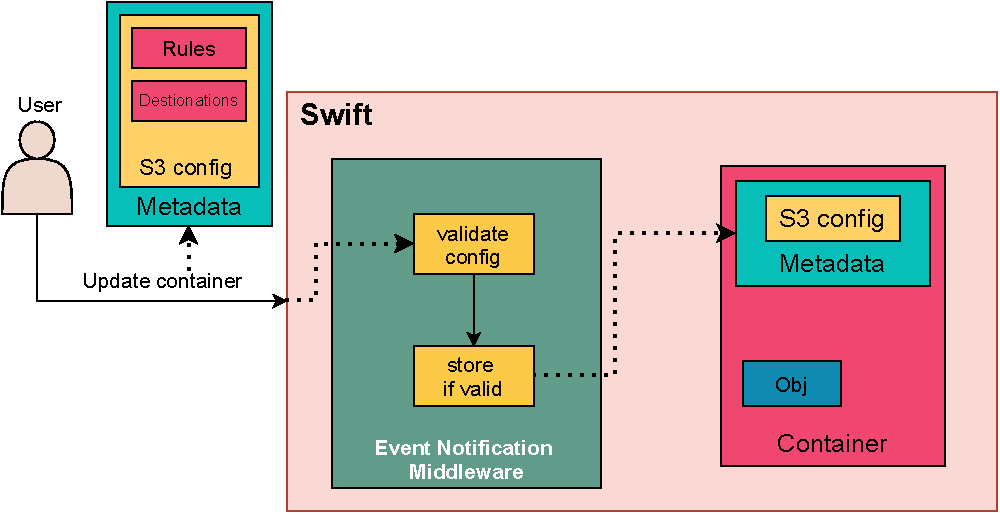
\includegraphics[width=0.90\linewidth]{images/swift-postconfiguration.pdf}
		\caption{Process of setting event notification configuration in ENOSS.}
		\label{fig:postConfiguration}
\end{figure}

\textbf{Reading stored event notification configuration} - Event notifications configuration can contain sensitive information. Since ENOSS stores configuration to storage using system metadata, which can be accessed only by application within OpenStack Swift, it disables reading stored configuration by simple GET/HEAD requests. For this purpose ENOSS offer API \\\centerline{\texttt{GET /v1/<acc>/<cont>?notification}}\\For security reasons, ENOSS allow only users with write rights to read stored configuration.

\textbf{Configuration structure} - Listing \ref{lst:eventConfiguration} describes event notification configuration. \texttt{<Target>} represent targeted destination where event notifications will be sent (e.g., Beanstalkd, Elasticsearch). \texttt{<FilterKey>} is a unique name of a filter containing rules that must be satisfied in order to publish events.

Event type takes form :\\\centerline{\texttt{s3:<Type><Action>:<Method>}}\\ and are compatible with Amazon S3 event types. Type represents resource type (object, bucket), action represent action preformed by user and can have values: \texttt{Created, Removed, Accessed}. The method represents the REST API method performed by a user: \texttt{Get, Put, Post, Delete, Copy, Head}. For example, if a new object was created, even type would be described as \texttt{s3:ObjectCreated:Put}. To match event type regardless of API method assign value \texttt{*} to \texttt{<Method>}.

\begin{lstlisting}[style=jsonStyle, caption=Strucute of event notification configuration,    label=lst:eventConfiguration]
{
  "<Target>Configrations": [
    {
      "Id": "configration id",
      "TargetParams": "set of key-value pairs, used specify dynamic parameters of targeted destination (e.g., name of beanstalkd tube or name of the index in Elasticsearch)",
      "Events": "array of event types that will be published",
      "PayloadStructure": "type of event notification structure: S3 or CloudEvents (default value S3)",
      "Filter": {
        "<FilterKey>": {
          "FilterRules": [
            {
              "Name": "filter operations (i.e. prefix, sufix, size)",
              "Value": "filter value"
            }
            ...
          ]
        }
      }
    }
    ...
  ]
}
\end{lstlisting}



\subsection{Interfaces}\label{sbs:intefaces}

One of the use cases of ENOSS can be publishing event notifications to custom destinations / currently unsupported destinations. In order to ease future development and support of new destinations, as well as different message structures and filters, ENOSS defined class interfaces and a set of rules needed to be followed in order to integrate new destination/message structure/filter to ENOSS.

\textbf{DestinationI} - is an interface specifying class that will be used for sending event notifications to the desired destination. The constructor receives configuration(dict), which can contain information needed for creating a connection with the desired destination(address, port, authentication,...). Configuration is loaded from ENOSS middleware configuration, which is loaded by the Proxy server. Method \texttt{send\_notification} receives notification(dict) and its task is to send notification to desired destination.

\begin{lstlisting}[language=Python, style=pythonStyle, caption=Interface of class used for sending notification message to desired destination, label=lst:enoss-destinationi]
class DestinationI(object, metaclass=abc.ABCMeta):
    @abc.abstractmethod
    def __init__(self, conf):
        raise NotImplementedError('__init__ is not implemented')

    @abc.abstractmethod
    def send_notification(self, notification):
        raise NotImplementedError('send_notification is not implemented')
\end{lstlisting}

\textbf{PayloadI} - is an interface specifying class that will be used for creating notification payload. When event notifications are configured on a container or account, ENOSS sends test notifications to all specified destinations in configuration. This way, it allows users to check if they successfully configured event notifications. Method \texttt{create\_test\_payload} is used for this purpose. One of the parameters is \texttt{request}, which contains all information about the incoming request(e.g., user IP address, incoming headers) as well as information about Swift response(e.g., headers, status code). \texttt{invoking\_configuration} contains informations about stored event notifications configuration. When an event occurs on a container/account with enabled event notifications, ENOSS checks if notification for such event should be published based on event notification configuration. If yes, method \texttt{create\_payload} will be used to create notification payload.

\begin{lstlisting}[language=Python, style=pythonStyle, caption=Interface of class used to create notification payload, label=lst:enoss-payloadi]
class PayloadI(object, metaclass=abc.ABCMeta):
    def __init__(self, conf):
        self.conf = conf

    @abc.abstractmethod
    def create_test_payload(self, app, request, invoking_configuration):
        raise NotImplementedError('create_test_payload is not implemented')

    @abc.abstractmethod
    def create_payload(self, app, request, invoking_configuration):
        raise NotImplementedError('create_payload is not implemented')
\end{lstlisting}

\textbf{RuleI} - is an interface specifying class that represents user-specified rule which must be satisfied in order to publish event notification. The constructor receives value, which is read from the event notification configuration. The call method has access to all information about the request, which allows implementing rules about, e.g., user IP address, return code, object prefix/suffix/length, etc.

\begin{lstlisting}[language=Python, style=pythonStyle, caption=Interface of class representing filter rule., label=lst:enoss-rulei]
class RuleI(object, metaclass=abc.ABCMeta):
    def __init__(self, value):
        self.value = value

    @abc.abstractmethod
    def __call__(self, app, request):
        raise NotImplementedError('__call__ is not implemented')
\end{lstlisting}

\subsection{Integration of new class implementing interface} - Often, implementation of new classes is way easier than its integration with a given system.

In the ENOSS case, where everything moves around event notifications configuration, which users specify, this problem can be challenging. ENOSS was designed with this problem in mind. In order to effortlessly integrate new classes that implement interfaces specified in \ref{sbs:intefaces}, several steps/rules must be followed:
\begin{itemize}
    \item \textbf{Class naming} - To integrate classes with ENOSS and allow users to use them in event notifications configuration, the class name must have a proper suffix. Name of classes implementing interface \texttt{DestinationI} must have suffix \texttt{Destination} (e.g. name of class sending notifications to Kafka would be \texttt{KafkaDestination}). Same principle applies for other interfaces, for payload suffix is \texttt{Payload} and for filter rule suffix is \texttt{Rule}
    \item \textbf{Names in event notifications configuration} - since class names in ENOSS must follow the above-specified rules, they are automatically integrated into ENOSS. Classes are connected with event notifications configuration using the class prefix name, i.e., without the class suffix described above.
\end{itemize}

In listing \ref{lst:eventConfigurationExample}, \texttt{KafkaConfigurations} means that class \texttt{KafkaDestination} will be used for sending notification, \texttt{"PayloadStructure": "S3"} means that \texttt{S3Payload} will be used for creating notification payload, and filter rule with \texttt{"Name": "suffix"} will use class \texttt{SuffixRule}.

\begin{lstlisting}[style=jsonStyle, caption=Example of event notifications configuration,    label=lst:eventConfigurationExample]
{
  "KafkaConfigurations": [
    {
      "Id": "kafka - example",
      "Events": "*",
      "PayloadStructure": "S3",
      "Filter": {
        "FilterExample": {
          "FilterRules": [
            {
              "Name": "suffix",
              "Value": ".jpg"
            }
          ]
        }
      }
    }
  ]
}
\end{lstlisting}

\section{Conclusions}
\label{sec:conclusions}


%\textbf{[Paper Summary]} What was the paper about, then? What the reader needs to remember about it?
This paper presents a solution for publishing notifications about events that occurred in OpenStack Swift.

%\textbf{[Highlights of Results]} Exact numbers. Remind the reader that the paper matters.
ENOSS is fully compatible with AWS S3 Event Notifications, offers multiple destinations to which notifications can be published, allows users to specify, using filters, which event notifications should be published. Furthermore, users can choose different types of notification payload (from standard AWS S3 payload structure to custom-defined structure) and offers a way for effortless expansions of new types of destinations, notification payloads, and filters.

%\textbf{[Paper Contributions]} What is the original contribution of this work? Two or three thoughts that one should definitely take home.
ENOSS can be used for monitoring events in OpenStack Swift, automatization and postprocessing, and serverless computing capable of reacting to events that occurred in OpenStack Swift(similarly to AWS Lambda).


%\textbf{[Future Work]} How can other researchers / developers make use of the results of this work? Do you have further plans with this work? Or anybody else?
In the future, new destinations(Elasticsearch, MySql, Redis, etc.) will be added. A further plan is the support of various new filters (filtering using time when an event occurred, stored metadata, etc.). Last but not least, support of different notification standards, such as CloudEvents.

\section*{Acknowledgements}\label{sec:ackn}
I would like to thank my supervisor RNDr. Marek Rychlý Ph.D. for his valuable advice and support during the creation of this work.


%--------------------------------------------------------
%--------------------------------------------------------
%--------------------------------------------------------
%	REFERENCE LIST
%--------------------------------------------------------
%--------------------------------------------------------
\phantomsection
\bibliographystyle{unsrt}
\bibliography{bibliography}

%--------------------------------------------------------
%--------------------------------------------------------
%--------------------------------------------------------
\end{document}
